\documentclass{article}

% ICLR 2027 submission. Double-blind: while \iclrfinalcopy (below) is commented out,
% the style automatically prints "Anonymous authors / Paper under double-blind review".
\usepackage{iclr2027_conference,times}

% Standard packages.
\usepackage[utf8]{inputenc}
\usepackage[T1]{fontenc}
\usepackage{hyperref}
\usepackage{url}
\usepackage{booktabs}
\usepackage{amsfonts}
\usepackage{nicefrac}
\usepackage{microtype}
\usepackage{xcolor}

% Project-specific packages used by figures and equations.
\usepackage{graphicx}
\usepackage{float}
\usepackage{amsmath, amssymb}
\usepackage{tikz}
\usetikzlibrary{shapes.geometric, arrows, positioning}

% Collect slack at the page bottom instead of stretching gaps between floats
% (tidies the float-heavy appendix pages).
\raggedbottom

\title{RLearner-LLM: Balancing Logical Grounding and Fluency in Large Language Models via Hybrid Direct Preference Optimization}

% Double-blind submission: anonymous author block. The style also prints
% "Anonymous authors / Paper under double-blind review" while \iclrfinalcopy is off.
% CAMERA-READY: uncomment \iclrfinalcopy (above) and restore the real author block.
\author{Anonymous authors}

%\iclrfinalcopy % Uncomment for the camera-ready/non-anonymous version to show real authors.

\begin{document}
\maketitle

\begin{abstract}
Direct Preference Optimization (DPO) has emerged as an efficient alternative to PPO-based RLHF, yet its application to knowledge-intensive generation tasks reveals a fundamental limitation: standard preference signals, whether from human annotators or LLM judges, exhibit a systematic \textit{verbosity bias} that rewards linguistic fluency over logical correctness. We show empirically that this reward signal blindspot leaves a large logical alignment gap: SFT-trained models achieve NLI entailment scores of only 0.05--0.22, despite producing fluent, confident-sounding text. We propose \textbf{RLearner-LLM}, a framework that resolves this through \textbf{Hybrid-DPO}: an automated preference construction pipeline that fuses a DeBERTa-v3 NLI entailment signal with a verifier LLM score, eliminating the need for human annotation while overcoming the ``alignment tax'' that degrades fluency under single-signal optimization. Evaluated across five academic domains (Biology, Medicine, Law) with three base architectures (LLaMA-2-13B, Qwen3-8B, and Gemma 4 E4B-it), RLearner-LLM achieves up to 6.6$\times$ NLI improvement over SFT baselines, with NLI gains in $11$ of $15$ (architecture, domain) cells and consistent answer-coverage gains. On Gemma 4 E4B-it, a 4.5B-effective-parameter dense model, Hybrid-DPO lifts NLI entailment in four of five domains (from +11.9\% on Auckland Law to +2.4$\times$ on UK Medicine Year 2), with faster inference across all five, demonstrating that the approach scales down to compact modern base models without losing the alignment-tax mitigation. We further show these gains are robust to aggressive, response-grounded question-quality filtering: under a \textit{strict-discriminator} filter that keeps only questions whose author key matches the modal student answer (computed from per-option student response logs), answer-coverage improves in every architecture--corpus cell and NLI in four of six. An independent held-out NLI scorer never used in training reproduces the SFT$\to$DPO improvement direction in $12$ of $15$ main cells, and a length-controlled follow-up shows a compact model can be preference-tuned toward better reasoning specifically: with a pairwise reasoning-quality reward and a length-normalised objective, its explanations are preferred over the SFT baseline by two independent judges ($70$--$72\%$) at matched output length. Our Qwen3-8B RLearner-LLM wins $95\%$ of blind pairwise comparisons against its own SFT baseline, while GPT-4o-mini in turn wins $95\%$ against our concise RLearner-LLM output, a result that, viewed alongside the $69\%$ win rate the same judge awards a verbose SFT baseline over our DPO-aligned model, reproduces the verbosity bias we document on a frontier comparator and reinforces the case for logic-aware automatic metrics (NLI, ACR) over LLM-as-a-judge on knowledge-intensive generation.\footnote{Code, training scripts, and per-domain evaluation artefacts (anonymised for review): \url{https://anonymous.4open.science/r/Explanation-Generation-468D/}}
\end{abstract}


\section{Introduction}

The generation of high-quality educational explanations represents a fundamental challenge in natural language processing. Unlike general-purpose conversational tasks, educational rationales must simultaneously satisfy two competing requirements: they must be \textit{logically grounded}, deriving the correct answer through sound deductive steps, and \textit{linguistically fluent}, maintaining natural, readable prose appropriate for a learner audience.

Supervised Fine-Tuning (SFT) on teacher-generated demonstrations has become the standard approach to instilling this capability into LLMs. However, SFT models exhibit a consistent and critical failure mode: while they produce fluent, confident-sounding text, they rarely construct the deductive chain that justifies \textit{why} the correct answer follows from the question context. Empirically, SFT models in our study achieve NLI entailment scores of only 0.05--0.22, indicating that the generated explanation rarely logically implies the ground-truth answer, even when the model ``knows'' the fact.

Reinforcement Learning from Human Feedback (RLHF) and its efficient derivative, Direct Preference Optimization (DPO) \citep{rafailov2023direct}, have sought to move beyond SFT by aligning models to human preferences. Yet these approaches contain a structural flaw when applied to factually demanding tasks: \textbf{the preference signal does not measure logical correctness}. Human annotators, and LLM judges, exhibit a well-documented \textit{verbosity bias}, systematically preferring longer, rhetorically polished responses over concise, logically precise ones \citep{zheng2024judging}. As we demonstrate empirically, GPT-4o-mini awards a 69\% win rate to a verbose SFT baseline over a more logically precise but concise RL-aligned model. DPO trained on such signals therefore reinforces stylistic fluency at the expense of factual grounding, leaving the core alignment gap unaddressed.

A natural remedy is to replace human preference labels with an automated logical metric, specifically, NLI entailment probability. However, optimizing DPO solely against NLI entailment incurs what we term the \textbf{alignment tax}: the model learns to produce short, repetitive snippets that satisfy the NLI scorer but collapse in linguistic coherence. This trade-off between logical soundness and readability represents a fundamental tension that single-dimensional reward signals cannot resolve.

\begin{figure}[h]
\centering
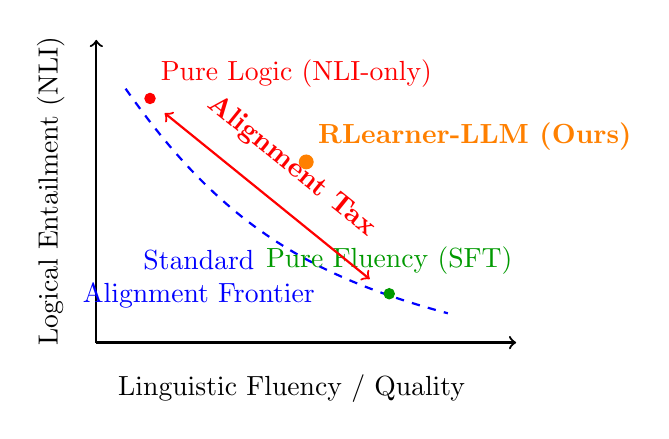
\begin{tikzpicture}[scale=0.62]
% Axes (titles placed clear of the plot to avoid label overlap)
\draw[->, thick] (0,0) -- (8.6,0);
\draw[->, thick] (0,0) -- (0,6.2);
\node[below] at (4.0,-0.45) {Linguistic Fluency / Quality};
\node[rotate=90, above] at (-0.45,3.1) {Logical Entailment (NLI)};

% Standard alignment frontier
\draw[blue, thick, dashed] (0.6,5.2) to[bend right=20] (7.2,0.6);
\node[blue, align=center] at (2.1,1.3) {Standard\\Alignment Frontier};

% Operating points (labels placed inward / above so none run off the axes)
\filldraw[red] (1.1,5.0) circle (3pt) node[above right=0.02cm] {Pure Logic (NLI-only)};
\filldraw[green!60!black] (6.0,1.0) circle (3pt) node[above=0.12cm] {Pure Fluency (SFT)};
\filldraw[orange] (4.3,3.7) circle (4pt) node[above right=0.04cm] {\textbf{RLearner-LLM (Ours)}};

% Alignment-tax trade-off arrow
\draw[<->, red, thick] (1.4,4.7) -- (5.6,1.3) node[pos=0.5, sloped, above=0.2cm] {\textbf{Alignment Tax}};

\end{tikzpicture}
\caption{Conceptual illustration of the \textbf{Alignment Tax}. Standard optimization forces a trade-off between logical grounding and linguistic fluency. RLearner-LLM pushes the Pareto frontier toward the upper-right quadrant through a dual-signal hybrid reward.}
\label{fig:alignment_tax}
\end{figure}

In this paper, we propose \textbf{RLearner-LLM}, a framework that resolves this tension by addressing the root cause directly: the reward signal used to construct preference pairs. Our key insight is that logical grounding and linguistic fluency are \textit{complementary objectives}, not competing ones, and that an automated dual-signal reward combining NLI entailment (for logical soundness) with a verifier score (for pedagogical quality) can construct high-fidelity preference pairs without human annotation, while simultaneously avoiding the degenerate solutions that plague single-signal optimization.

Our contributions are as follows:
\begin{enumerate}
    \item \textbf{Problem diagnosis}: We identify that the root cause of logical misalignment in DPO-trained educational models is not the optimization algorithm itself, but the \textit{reward signal blindspot}: the inability of standard preference signals to measure logical correctness. We provide empirical evidence of verbosity bias in LLM-as-a-judge evaluation that perpetuates this blindspot.
    \item \textbf{Hybrid-DPO framework}: We introduce \textbf{RLearner-LLM}, which automatically constructs preference pairs $\mathcal{D}_{pref}$ using a composite score $H(E_i) = 0.5\cdot S_{\text{NLI}}(E_i) + 0.5\cdot \tilde{S}_{\text{Verifier}}(E_i)$, fusing a DeBERTa-v3 NLI signal with a min-max-normalised verifier LLM score (Eq.~\ref{eq:hybrid_reward}). The dual-signal hybrid eliminates the need for human annotation while overcoming the alignment tax.
    \item \textbf{Cross-architecture validation}: We validate across three base architectures (LLaMA-2-13B, Qwen3-8B, and Gemma 4 E4B-it) and five academic domains (Biology, Medicine, Law), demonstrating up to 6.6$\times$ NLI improvement over SFT baselines in $11$ of $15$ (architecture, domain) cells, with consistent ACR gains on stronger base models. Gemma 4 E4B-it, a 4.5B-effective-parameter dense model, shows Hybrid-DPO NLI gains in four of five domains (+11.9\% Auckland Law, +32.0\% UK Medicine Y1, +65.6\% Cardiff Biology, +2.4$\times$ UK Medicine Y2), with faster inference across all five and the first single-pass-RL result to surpass the iterative ILearner-LLM (K=5) baseline on Auckland Law NLI. Our Qwen3-8B model further wins $95\%$ of blind pairwise comparisons against its own SFT baseline; on the same judge it loses $95\%$ to GPT-4o-mini's longer outputs, replicating the verbosity bias on a frontier comparator and motivating logic-aware automatic metrics over LLM-as-a-judge for knowledge-intensive generation.
    \item \textbf{Robustness to question-quality filtering}: Using the full PeerWise answer-submission logs, we show the gains survive a \textit{strict-discriminator} filter that keeps only questions whose author key matches the \emph{modal student answer}: across three architectures and two corpora, answer-coverage improves in all six (architecture, corpus) cells and NLI in four of six, reproducing the per-architecture pattern of the main results (Appendix~\ref{sec:tierc_appendix}).
    \item \textbf{Independent validation and a step toward reasoning}: An out-of-training held-out NLI scorer (DeBERTa-v3-large) reproduces the improvement direction in $12$ of $15$ main cells, evidence against reward-hacking of the training scorer. Going beyond entailment, we build a pairwise reasoning-quality reward and, using a length-normalised objective, obtain a compact model whose explanations two independent judges prefer over the SFT baseline ($70$--$72\%$ of non-tied pairs) \emph{at matched output length}, indicating the gain is genuine reasoning quality rather than verbosity (\S\ref{sec:reasoning-reward}, Appendix~\ref{sec:reasoning_appendix}).
\end{enumerate}

\section{Related Work}
\label{sec:related_work}

\subsection{Alignment and Preference Optimization}
Optimizing Large Language Models (LLMs) to align with human intent has predominantly relied on Reinforcement Learning from Human Feedback (RLHF) \citep{ouyang2022training}, utilizing Proximal Policy Optimization (PPO) \citep{schulman2017proximal}. Recently, Direct Preference Optimization (DPO) \citep{rafailov2023direct} emerged as a stable alternative that mathematically bypasses the need for an explicit reward model. Building on this, recent advancements like RRHF \citep{yuan2023rrhf}, ORPO \citep{hong2024orpo}, and SimPO \citep{meng2024simpo} have further simplified alignment via reference-free objectives. Recent work adds adaptive batch-wise scheduling \citep{zhang2025adaptive} and constrained-alignment methods \citep{chen2025constrained}, addressing algorithmic biases in RLHF \citep{ji2024limits, shrivastava2024algorithmic}. A parallel line \emph{unifies} SFT and RL into a single objective \citep{liu2025uft, wang2024uft}; our contribution is orthogonal and composable with it, keeping the standard SFT$\to$DPO pipeline and changing only how preference pairs are labelled. Like RLAIF \citep{lee2023rlaif} our labels need no human annotation; unlike it, they come from an NLI model or a pairwise reasoning judge rather than a general-purpose LLM preference.
\subsection{Reasoning Quality and Faithfulness Rewards}
Rewarding the logical quality of a generation, rather than human preference, has been studied with process-based feedback \citep{uesato2023verify}, checks on decision pivots in chain-of-thought \citep{wang2025pivots}, and entailment rewards for summarisation faithfulness \citep{pasunuru2018multireward, roit2023factually}. Retrieval \citep{lewis2020retrieval} and hallucination detection \citep{li2023haludetect} target factual errors; we do not address hallucination beyond reporting how often SFT outputs contain fabricated URLs. Our concern is narrower: whether an entailment reward measures reasoning or can be met by restating the answer, a risk also noted for metric-driven evaluation generally \citep{schaeffer2023mirage}.

\subsection{LLM-as-a-Judge and Evaluation Bias}
The use of powerful instruction-tuned models like GPT-4 as automated evaluators \citep{zheng2024judging} is widespread but prone to significant biases, including verbosity bias \citep{wang2023large} and self-preference bias \citep{pan2024evalbias}. The verbosity-bias confound has been formally analysed in DPO itself: \citep{park2024lengthbias} show that standard DPO and its $\beta$-tuned variants \citep{park2024betadpo} systematically conflate explanation length with quality, and propose length-aware regularisation as a partial remedy. We avoid LLM-judge labels for training the NLI-reward policies, and where we use LLM judges for evaluation we compare outputs of matched length and use several judges from different model families. Table~\ref{tab:pairwise_1} shows that, without such controls, a GPT-4o-mini judge picks the longer of two outputs in every comparison we ran.

% NeurIPS Best Paper Style – clean, flat, minimal
\definecolor{NBlue}{HTML}{1A56A0}
\definecolor{NRed}{HTML}{C0392B}
\definecolor{NGreen}{HTML}{1A7A45}
\definecolor{NGold}{HTML}{B07D1A}
\definecolor{NSlate}{HTML}{4A5568}
\definecolor{NBlueFill}{HTML}{EBF2FB}
\definecolor{NRedFill}{HTML}{FBEAEA}
\definecolor{NGreenFill}{HTML}{EBF5EF}
\definecolor{NGoldFill}{HTML}{FDF6E3}
\definecolor{NSlateFill}{HTML}{F0F2F5}
\definecolor{NStroke}{HTML}{BBBDC2}

\begin{figure}[t!]
\centering
\begin{tikzpicture}[
    scale=0.88,
    >=stealth,
    % Core node styles
    iobox/.style={
        draw=NStroke, fill=NSlateFill,
        rounded corners=4pt, align=center,
        font=\small, inner sep=7pt, line width=0.6pt
    },
    modbox/.style={
        draw=#1, fill=#1Fill,
        rounded corners=5pt, align=center,
        font=\small\bfseries, inner sep=7pt,
        minimum height=1.0cm, minimum width=3.2cm,
        line width=0.7pt
    },
    rewardbox/.style={
        draw=NGold, fill=NGoldFill,
        rounded corners=5pt, align=center,
        font=\footnotesize, inner sep=10pt,
        minimum height=1.7cm, minimum width=11.0cm,
        line width=0.7pt
    },
    dpobox/.style={
        draw=NBlue, fill=NBlueFill,
        rounded corners=5pt, align=center,
        font=\small\bfseries, inner sep=8pt,
        minimum height=1.0cm, minimum width=9.0cm,
        line width=0.8pt
    },
    arr/.style={->, line width=0.7pt, color=NSlate, shorten >=3pt, shorten <=3pt},
    arrd/.style={->, line width=0.7pt, color=NBlue!50, dashed, shorten >=3pt, shorten <=3pt},
    steplabel/.style={font=\footnotesize\bfseries, color=NSlate},
    sublabel/.style={font=\scriptsize, color=NSlate!80}
]

%%,,,,,,,,, -
%% STAGE 1 background (subtle)
\draw[draw=NStroke!50, fill=NSlateFill!40, rounded corners=8pt, line width=0.5pt, dashed]
    (-5.6, 2.8) rectangle (5.6, 5.0);
\node[sublabel, anchor=north west] at (-5.5, 4.95) {Stage 1: Stochastic Generation};

%% STAGE 1: Input → Generator → Candidates
\node[iobox] (input) at (-3.8, 3.9) {Context\\$(C,\, Q)$};
\node[modbox=NBlue] (gen) at (0, 3.9) {Generator\\$\pi_{\theta}$};
\node[iobox] (cands) at (3.8, 3.9) {Explanations\\$\mathcal{E} = \{E_i\}_{i=1}^{n}$};

\draw[arr] (input) -- (gen);
\draw[arr] (gen) -- node[above, sublabel, yshift=1pt] {$n$ samples} (cands);

%%,,,,,,,,, -
%% STAGE 2 background
\draw[draw=NStroke!50, fill=NSlateFill!30, rounded corners=8pt, line width=0.5pt, dashed]
    (-5.6, -4.85) rectangle (5.6, 2.5);
\node[sublabel, anchor=north west] at (-5.5, 2.45) {Stage 2: Logic-Driven Reward \& Alignment};

%% Fan-out connector
\draw[arr] (cands.south) -- ++(0,-0.6) coordinate (fanout);
\draw[arr] (fanout) -- (-3.6, 1.4);
\draw[arr] (fanout) -- (0,   1.4);
\draw[arr] (fanout) -- ( 3.6, 1.4);

%% REWARD COMPONENTS
\node[modbox=NRed,   minimum width=3.0cm] (nli) at (-3.6, 0.7)
    {NLI Entailment\\$S_{\text{nli}}(E_i)$};
\node[modbox=NGreen, minimum width=3.0cm] (ver) at (0,    0.7)
    {Stylistic Verifier\\$S_{\text{ver}}(E_i)$};
\node[modbox=NSlate, minimum width=3.0cm] (len) at ( 3.6, 0.7)
    {Length Penalty\\$\gamma\,\ell(E_i)$};

%% Converge arrows toward reward-box top (top edge at y=-0.9)
\draw[arr] (nli.south) -- ++(0,-0.3) -| (-2.5,-0.8);
\draw[arr] (ver.south) -- ++(0,-0.3) -- (0,-0.8);
\draw[arr] (len.south) -- ++(0,-0.3) -| ( 2.5,-0.8);

%% HYBRID REWARD (two operating points: A = additive, M = multiplicative ACR)
\node[rewardbox] (reward) at (0, -1.75)
    {{\small\bfseries Hybrid Reward}\;\;{\scriptsize\itshape (additive A or multiplicative-ACR M, selected per training pool)}\\[3pt]
     \makebox[1.45cm][r]{\textbf{\textcolor{NGold!85!black}{(A)}}\,}\,$H_A(E_i) \;=\; 0.5\,S_{\text{nli}}(E_i) \;+\; 0.5\,\tilde{S}_{\text{ver}}(E_i)$\\[1.5pt]
     \makebox[1.45cm][r]{\textbf{\textcolor{NGold!85!black}{(M)}}\,}\,$H_M(E_i) \;=\; \bigl(w_{\text{nli}}\,S_{\text{nli}}\,\cdot\,w_{\text{ver}}\,\tilde{S}_{\text{ver}} \;-\; \gamma\,\ell\bigr)\;\cdot\;\mathbf{1}\!\bigl[\mathrm{acr}(E_i)\geq\theta\bigr]$};

%% Reward → DPO
\draw[arr] (reward.south) -- node[right, sublabel, xshift=3pt] {reward signal} ++(0,-0.55) coordinate (mid);
\draw[arr] (mid) -- ++(0,-0.3);

\node[dpobox] (dpo) at (0, -4.1)
    {Hybrid Direct Preference Optimisation (Hybrid-DPO)};

%% FEEDBACK LOOP
\draw[arrd]
    (dpo.west)
    .. controls (-7.2, -4.1) and (-7.2, 3.9) ..
    (gen.west)
    node[midway, sloped, above, font=\scriptsize\bfseries, color=NBlue!60]
        {preference update};

\end{tikzpicture}
\caption{The \textbf{RLearner-LLM} framework. Stage~1 samples $n$ candidates from $\pi_\theta$; Stage~2 scores each with the dual-signal \textbf{Hybrid Reward}, either the additive $H_A$ or the multiplicative-ACR $H_M$ (\S\ref{sec:first_principles}; selector: pool $\geq{\sim}150$ pairs and a single/aligned domain $\to H_M$, else $H_A$). NLI and verifier feed both variants; the length penalty and ACR gate $\mathbf{1}[\mathrm{acr}\geq\theta]$ enter $H_M$ only. Preference pairs then update $\pi_\theta$ via Hybrid-DPO. $\tilde{S}_{\text{ver}}{=}(S_{\text{ver}}{-}1)/4$ is the $[0,1]$-normalised verifier score.}
\label{fig:hybrid_dpo}
\end{figure}

\section{Methodology}
\label{sec:methodology}

\subsection{First-Principles Derivation of the Hybrid Reward}
\label{sec:first_principles}

\paragraph{The RLHF Objective and Its Core Tension.}
The canonical RLHF objective~\citep{ouyang2022training} is:
\begin{equation}
\max_{\pi_\theta}\; \mathbb{E}_{y \sim \pi_\theta(y|x)}\bigl[r(x,y)\bigr] - \beta\,\text{KL}\bigl(\pi_\theta \,\|\, \pi_\text{ref}\bigr)
\label{eq:rlhf}
\end{equation}
where $\pi_\text{ref}$ is the supervised fine-tuned reference policy and $\beta$ controls how much the learned policy is allowed to deviate from it.
DPO~\citep{rafailov2023direct} derives the closed-form optimal policy
$\pi^*(y|x) \propto \pi_\text{ref}(y|x)\cdot\exp(r(x,y)/\beta)$ and reformulates the objective as a direct binary cross-entropy loss on preference pairs, eliminating the need for an explicit reward model.

The \textbf{alignment tax} arises from a \emph{gradient conflict}: the KL term in Eq.~\ref{eq:rlhf} regularises $\pi_\theta$ toward an MLE-trained $\pi_\text{ref}$ that prefers verbose, surface-coherent text, while a logic-focused reward (e.g.\ pure NLI entailment) rewards short dense deductive chains off that fluency manifold. Single-signal optimisation under this conflict either collapses into degenerate snippets that satisfy NLI at the cost of coherence, or capitulates to the KL prior and produces fluent-but-logically-weak text, both manifest as alignment tax on the frontier in Fig.~\ref{fig:alignment_tax}.

\paragraph{The Dual-Signal Hybrid Reward.}
The load-bearing design choice is to score candidates with both an NLI entailment score $S_\text{NLI}(E)\in[0,1]$ and a min-max-normalised verifier score $\tilde{S}_\text{ver}(E){=}(S_\text{ver}(E){-}1)/4\in[0,1]$. Used alone each signal degenerates (pure NLI yields answer-repeating snippets; pure verifier reintroduces verbosity bias \citep{wang2023large,park2024lengthbias}). We instantiate the Hybrid reward at two operating points:
\begin{subequations}
\label{eq:hybrid_reward}
\begin{align}
H_A(E) &= 0.5\,S_\text{NLI} + 0.5\,\tilde{S}_\text{ver}, \label{eq:hybrid_add}\\
H_M(E) &= \bigl(w_\text{nli}\,S_\text{NLI}\cdot w_\text{ver}\,\tilde{S}_\text{ver} - \gamma\,\ell_\text{norm}\bigr)\cdot\mathbf{1}[\mathrm{ACR}{\geq}\theta]. \label{eq:hybrid_mult}
\end{align}
\end{subequations}
The additive $H_A$ (Eq.~\ref{eq:hybrid_add}) admits chosen pairs when \emph{either} signal is sufficiently better than the rejected counterpart (high recall). The multiplicative-ACR $H_M$ (Eq.~\ref{eq:hybrid_mult}) requires \emph{both} signals to favour the chosen candidate via the product, hard-gates on $\mathrm{ACR}(E){\geq}\theta$ to drop answer-evasive candidates, and subtracts a length penalty $\gamma\,\ell_\text{norm}(E)$ to suppress the length confounder (high precision). $H_A$ contains no length term: in cross-domain pools the heterogeneous length distribution destabilises a single $\gamma$, and $H_A$ is preferred precisely there.

\paragraph{Selector rule.}
$H_M$ retains $\sim\!2$--$4\times$ fewer preference pairs than $H_A$ on the same candidate pool (the hard gate drops ${\sim}40\%$ of candidates, and the product collapses many surviving pairs below the score-gap threshold). We default to $H_M$ and fall back to $H_A$ when the projected $H_M$ pool drops below ${\sim}150$ pairs or the training corpus merges domains with disparate answer-keyword distributions. This rule is post-hoc rationalisation of our experimental progression; the head-to-head Table~\ref{tab:variant_ablation} shows $H_A$ and $H_M$ within ${\sim}1$\,pp NLI on average across $11$ matched cells, $H_M$ winning $7/11$. The dual-signal $H_M$ beats both single-signal ablations on Qwen3-8B Cardiff (SFT $0.1959$) --- NLI-only ($0.1419$) and verifier-only ($0.1368$) --- while $H_A$ is within noise of NLI-only there; the dual-signal hypothesis, not the algebraic form, is the load-bearing claim.

\subsection{Preference Pair Construction}
\label{sec:pref_construction}

Given $n$ candidate explanations $\{E_i\}_{i=1}^n$ sampled from $\pi_\theta$ for $(C, Q)$, we score each with $H(E_i)$ and retain pairs $(E_i, E_j)$ with $H(E_i) > H(E_j) + \Delta$ as (chosen, rejected), where $\Delta{\geq}0.05$. Under $H_M$, the ACR gate is a hard pre-filter: only pairs whose chosen member passes $\mathrm{ACR}{\geq}\theta$ are eligible, ruling out the rank-inversion edge case where a long but valid candidate could receive $H_M(E){<}0$ from the length penalty (we verified empirically that this corner case produces no inversions in our 5-domain pool).

\subsection{Hybrid-DPO Training Objective}
\label{sec:hybrid_dpo}

The Hybrid-DPO objective follows the standard DPO formulation~\citep{rafailov2023direct} but is trained on $\mathcal{D}_\text{pref}$ constructed with the Hybrid reward (Eq.~\ref{eq:hybrid_reward}):
\begin{equation}
\mathcal{L}_\text{DPO}(\pi_\theta) = -\mathbb{E}_{(x,y^+,y^-)\sim\mathcal{D}_\text{pref}}\!\left[\log\sigma\!\left(\beta\!\left(\log\frac{\pi_\theta(y^+|x)}{\pi_\text{ref}(y^+|x)} - \log\frac{\pi_\theta(y^-|x)}{\pi_\text{ref}(y^-|x)}\right)\right)\right]
\label{eq:dpo_loss}
\end{equation}
Because every chosen example $y^+$ in $\mathcal{D}_\text{pref}$ outscores its rejected counterpart on \emph{both} dual-signal axes, NLI entailment and verifier fluency, regardless of which Hybrid variant ($H_A$ or $H_M$) constructed the pair, the gradient of $\mathcal{L}_\text{DPO}$ consistently points toward higher logical entailment without sacrificing pedagogical quality. This is the mechanism by which the Hybrid reward breaks the fluency attractor that causes alignment tax in single-signal optimisation.

\paragraph{Implementation notes.}
Two base models in this study require non-default LoRA target selection. Qwen3-8B applies RMSNorm to $q,k$ after the projection reshape, so LoRA adapters on \texttt{q\_proj}/\texttt{k\_proj} would corrupt that path; we restrict its targets to \texttt{v\_proj}, \texttt{o\_proj}, and the three MLP projections. Gemma 4 E4B-it ships as a multimodal \texttt{Gemma4ForConditionalGeneration} checkpoint whose text-tower weights live under \texttt{model.language\_model.*}; we therefore load that class explicitly and use a full-path LoRA target regex that matches exactly the $258$ plain \texttt{nn.Linear} attention/MLP projections in the text tower (full pattern in Appendix~\ref{sec:impl_notes_appendix}). At inference, the DPO adapter must be composed on top of the SFT-merged base ($\text{base}\to\text{apply SFT}\to\text{merge}\to\text{apply DPO}\to\text{merge}$), since the DPO delta was trained relative to that reference point.

\section{Experimental Setup}
\label{sec:experimental_setup}
\label{sec:setup}

\textbf{Models.} LLaMA-2-13B, Qwen3-8B and Gemma~4 E4B-it (4.5B effective parameters), each fine-tuned with LoRA ($r{=}16$, $\alpha{=}32$, 3 epochs) on 13{,}211 student-written PeerWise explanations \citep{bao2025exploring} pooled from five courses: Cardiff Biology, Sydney Biology, Auckland Law, and UK Medicine Years 1 and 2.

\textbf{Preference data.} For each base model we sample $n{=}3$ explanations for 500 training questions drawn from the same pooled corpus, so every pool contains questions from all five courses (Appendix~\ref{sec:pair_stats}); no pool shares a question with a test set. We keep the best- vs.\ worst-scoring pair when the score gap is $\geq 0.05$, which leaves 143--632 pairs. DPO: 5 epochs, lr $5{\times}10^{-5}$, $\beta{=}0.1$, effective batch 8.

\textbf{Test sets and decoding.} Each course has a fixed 100-question test set. Qwen3 and Gemma~4 decode greedily. The LLaMA-2 harness samples ($T{=}0.5$), so the same LLaMA-2 SFT checkpoint scores differently from run to run (e.g.\ Cardiff NLI 0.045--0.21 over 11 runs, Appendix~\ref{sec:provenance}). We therefore always compare a DPO policy with the SFT row of the \emph{same} evaluation run, and report a 95\% bootstrap confidence interval for the change. We have one DPO training seed per cell; the SimPO result of \S\ref{sec:reasoning-reward} has three.

\textbf{Metrics.} \emph{NLI}: $S_\text{NLI}$ with the training scorer. \emph{Held-out NLI}: the same with \texttt{cross-encoder/nli-deberta-v3-large}, which is used nowhere in training, pair construction or model selection. \emph{Copies}: the share of explanations that contain the correct-option text verbatim. ACR, BLEU, BERTScore and the verifier score are in Appendix~\ref{sec:per_domain_appendix}.

\textbf{Answer-masking test.}\label{sec:masking} An explanation can entail the answer by restating it. To see how much entailment remains without that, we replace, in the explanation, the full option text and every word beginning with one of the option's key terms (words of $\geq$4 letters) with \texttt{[MASK]}, and re-score with the held-out model. For example, with the option ``ATP is generated anaerobically through substrate level phosphorylation using creatine phosphate'', the explanation sentence ``ATP is generated anaerobically \ldots'' becomes ``[MASK] is [MASK] [MASK] \ldots'', while the reasons around it are kept. Masked scores are low for every model; what matters is whether DPO raises or lowers them relative to SFT.

\section{Results}
\label{sec:results}

\subsection{Entailment gains, and what they are made of}
\label{sec:main_results}

\begin{table}[t]
\centering
\caption{SFT$\to$RLearner-LLM on the five test sets. Each pair of numbers comes from \emph{one} evaluation run on the same 100 questions (LLaMA-2 decodes by sampling at $T{=}0.5$, so its SFT score varies between runs; Qwen3 and Gemma~4 decode greedily). \emph{NLI}: training scorer (DeBERTa-v3-small), bold if the 95\% bootstrap CI of the change excludes zero. \emph{Held-out}: DeBERTa-v3-large, used nowhere in training. \emph{Masked}: held-out NLI after every key term of the correct option is replaced by \texttt{[MASK]} in the explanation (\S\ref{sec:masking}); bold marks an increase. \emph{Copies}: \% of explanations containing the correct-option text verbatim.}
\label{tab:main}
\resizebox{\textwidth}{!}{%
\begin{tabular}{llcccccc}
\toprule
Model & Test set & NLI & 95\% CI of $\Delta$ & Held-out NLI & Masked held-out NLI & Words & Copies (\%) \\
\midrule
LLaMA-2-13B & Cardiff Bio. & \textbf{.082$\to$.319} & [+0.14, +0.33] & \textbf{.308$\to$.383} & .198$\to$.104 & 228$\to$80 & 54$\to$71 \\
LLaMA-2-13B & Sydney Bio. & \textbf{.069$\to$.356} & [+0.19, +0.38] & \textbf{.179$\to$.464} & .104$\to$.065 & 288$\to$55 & 37$\to$61 \\
LLaMA-2-13B & Auckland Law & .289$\to$.323 & [-0.07, +0.14] & .520$\to$.376 & .283$\to$.132 & 191$\to$80 & 46$\to$60 \\
LLaMA-2-13B & UK Med Y1 & \textbf{.069$\to$.425} & [+0.26, +0.45] & \textbf{.254$\to$.455} & .149$\to$.124 & 223$\to$69 & 57$\to$74 \\
LLaMA-2-13B & UK Med Y2 & \textbf{.076$\to$.388} & [+0.21, +0.41] & \textbf{.198$\to$.430} & .144$\to$.079 & 215$\to$74 & 49$\to$75 \\
\midrule
Qwen3-8B & Cardiff Bio. & .196$\to$.182 & [-0.11, +0.08] & .281$\to$.238 & \textbf{.071$\to$.141} & 59$\to$181 & 59$\to$78 \\
Qwen3-8B & Sydney Bio. & .174$\to$.231 & [-0.04, +0.15] & .320$\to$.290 & \textbf{.067$\to$.156} & 66$\to$179 & 40$\to$71 \\
Qwen3-8B & Auckland Law & .319$\to$.230 & [-0.20, +0.02] & \textbf{.297$\to$.409} & \textbf{.071$\to$.221} & 32$\to$199 & 41$\to$85 \\
Qwen3-8B & UK Med Y1 & .246$\to$.207 & [-0.13, +0.06] & .315$\to$.258 & \textbf{.081$\to$.162} & 56$\to$184 & 65$\to$75 \\
Qwen3-8B & UK Med Y2 & .163$\to$.207 & [-0.05, +0.13] & \textbf{.202$\to$.255} & \textbf{.073$\to$.151} & 74$\to$182 & 44$\to$75 \\
\midrule
Gemma~4 E4B & Cardiff Bio. & \textbf{.212$\to$.350} & [+0.03, +0.25] & \textbf{.239$\to$.400} & \textbf{.060$\to$.105} & 61$\to$45 & 57$\to$53 \\
Gemma~4 E4B & Sydney Bio. & .247$\to$.231 & [-0.12, +0.09] & .414$\to$.355 & \textbf{.081$\to$.110} & 61$\to$49 & 44$\to$38 \\
Gemma~4 E4B & Auckland Law & .391$\to$.438 & [-0.08, +0.17] & \textbf{.349$\to$.454} & \textbf{.057$\to$.083} & 29$\to$28 & 46$\to$48 \\
Gemma~4 E4B & UK Med Y1 & .296$\to$.391 & [-0.02, +0.21] & \textbf{.266$\to$.502} & \textbf{.042$\to$.106} & 55$\to$40 & 66$\to$51 \\
Gemma~4 E4B & UK Med Y2 & \textbf{.160$\to$.389} & [+0.12, +0.33] & \textbf{.264$\to$.412} & \textbf{.069$\to$.083} & 67$\to$54 & 49$\to$47 \\
\bottomrule
\end{tabular}}
\end{table}


Table~\ref{tab:main} gives the 15 (model, test set) cells; Figure~\ref{fig:masking} plots the held-out and masked changes. The three base models behave differently.

\textbf{LLaMA-2-13B: the gain is restatement.} Entailment rises in four of five test sets with confidence intervals well above zero (e.g.\ UK Med Y1 0.069$\to$0.425), and the held-out scorer agrees. But DPO also cuts the output from 190--290 to 55--80 words and raises the share that copies the answer (e.g.\ 49\%$\to$75\% on Med Y2). Once the answer is masked, the held-out score is \emph{lower} than SFT's in all five test sets. The model has learned to state the answer in a short output, not to argue for it. Auckland Law, the one non-significant cell, is also where ILearner-LLM, which refines each answer five times, stays ahead (Appendix~\ref{sec:per_domain_appendix}).

\textbf{Qwen3-8B: no reliable change.} No confidence interval excludes zero, the two scorers disagree on direction in two cells, and outputs triple in length (32--74$\to$179--199 words). The masked score rises, but with three times as much text to mask around we do not read this as evidence either way.

\textbf{Gemma~4 E4B: a gain that survives masking.} The held-out scorer improves in four of five test sets (all but Sydney) and the masked score in all five, while outputs get \emph{shorter} (by 1--16 words) and copy the answer no more often (change $-15$ to $+2$ points). The training-scorer change has a CI above zero on Cardiff and Med Y2; on Med Y1 and Law the CI touches zero. This is the result we consider robust: on Gemma~4, the entailment reward improves how well the explanation supports the answer beyond repeating it. Whether reasoning judges also prefer these outputs is a separate question, which \S\ref{sec:single_dual} answers in the negative. On the strict question-quality filter of Appendix~\ref{sec:tierc_appendix} the Gemma~4 gains are larger (held-out 0.32$\to$0.56 on Cardiff, 0.37$\to$0.55 on Sydney).

Across all 15 cells, the CI excludes zero in 6, a one-sided paired Wilcoxon test gives $p{<}0.05$ in 9, and the two scorers agree on the direction of the change in 12.

\subsection{Does combining NLI with a verifier help?}
\label{sec:single_dual}
\label{sec:variant_ablation}

\begin{table}[t]
\centering
\caption{Gemma~4: every reward variant trained on pairs drawn from \emph{one} shared pool (500 prompts $\times$ 3 candidates, each scored once by every signal), with identical DPO settings. Means over the five test sets (500 questions, greedy decoding). Rows with $\pm$ give mean$\pm$s.d.\ over three DPO seeds; all other cells are seed 42. The CI is a paired bootstrap of the seed-42 change in masked held-out NLI vs.\ SFT. Ver: \emph{reproduced} verifier (Appendix~\ref{sec:verifier_repro}). Judge: \% of non-tie pairwise reasoning judgements won against SFT (Qwen2.5-7B / Llama-3.1-8B / Gemma-4-31B, 500 items each, order-flipped). Round-2 SimPO rows use $\beta{=}2$, $\gamma{=}1$, 3 epochs; the reasoning-judge reward is a fourth model (Qwen3-8B) that is never used for evaluation. Judge cells of three-seed rows pool the three seeds' judgements.}
\label{tab:g4shared}
\resizebox{\textwidth}{!}{%
\begin{tabular}{lccccccccc}
\toprule
Reward & Pairs & NLI & Held-out NLI & Masked held-out & 95\% CI $\Delta$masked & Words & Copies (\%) & Ver & Judge vs SFT \\
\midrule
SFT & -- & 0.261 & 0.307 & 0.062 & -- & 55 & 52 & 2.89 & -- \\
\midrule
Verifier only & 314 & 0.160 & 0.266 & 0.086 & [+0.001, +0.048] & 99 & 51 & 3.18 & -- \\
$H_A$, $w{=}0.25$ & 258 & 0.287 & 0.397 & 0.087 & [+0.003, +0.047] & 66 & 54 & 3.00 & -- \\
$H_A$, $w{=}0.5$ & 257 & 0.335 & 0.435 & 0.103 & [+0.019, +0.064] & 62 & 52 & 2.95 & -- \\
$H_A$, $w{=}0.75$ & 262 & 0.331 & 0.425 & 0.100 & [+0.016, +0.060] & 57 & 51 & 2.92 & -- \\
NLI only & 270 & 0.381 & 0.473 & 0.133 & [+0.048, +0.095] & 53 & 47 & 2.89 & 39 / 42 / 41 \\
$H_M$ (Table~\ref{tab:main} reward) & 159 & 0.311$\pm$0.011 & 0.405$\pm$0.015 & 0.086$\pm$0.006 & [+0.008, +0.047] & 49 & 50 & 2.89 & 38 / 41 / 39 \\
$H_M$, dominating pairs only & 117 & 0.270 & 0.334 & 0.080 & [-0.002, +0.038] & 60 & 53 & 2.94 & -- \\
Masked NLI & 93 & 0.272$\pm$0.006 & 0.343$\pm$0.011 & 0.084$\pm$0.007 & [-0.002, +0.036] & 58 & 54 & 2.91 & 47 / 47 / 47 \\
NLI only, 93 random pairs & 93 & 0.277$\pm$0.010 & 0.361$\pm$0.004 & 0.083$\pm$0.010 & [-0.004, +0.033] & 56 & 54 & 2.88 & 46 / 53 / 53 \\
\midrule
\multicolumn{10}{l}{\emph{Round 2: lighter NLI training, SimPO, and a reasoning-judge reward (Qwen3-8B) on the same pool}} \\
NLI only, 1 epoch & 270 & 0.240 & 0.300 & 0.077 & [+0.004, +0.028] & 54 & 55 & 2.89 & 50 / 49 / 52 \\
NLI only, 2 epochs & 270 & 0.310 & 0.351 & 0.077 & [+0.001, +0.029] & 50 & 53 & 2.89 & 49 / 48 / 47 \\
NLI only, $\beta{=}0.5$ & 270 & 0.287 & 0.339 & 0.085 & [+0.005, +0.041] & 53 & 54 & 2.90 & 48 / 49 / 50 \\
NLI only (SimPO) & 270 & 0.391 & 0.403 & 0.092 & [+0.009, +0.053] & 29 & 44 & 2.84 & 39 / 36 / 31 \\
Reasoning judge (SimPO) & 293 & 0.244 & 0.313 & 0.084 & [+0.001, +0.045] & 60 & 45 & 2.90 & 48 / 60 / 61 \\
Judge + NLI (SimPO) & 390 & 0.343 & 0.410 & 0.115 & [+0.028, +0.078] & 48 & 47 & 2.86 & 42 / 47 / 40 \\
\midrule
\multicolumn{10}{l}{\emph{Round 3: judge pairs restricted to candidates within 15 words of each other}} \\
Judge, length-matched pairs (SimPO) & 182 & 0.258$\pm$0.011 & 0.316$\pm$0.000 & 0.075$\pm$0.001 & [-0.006, +0.030] & 54 & 52 & 2.88 & 52 / 56 / 54 \\
Judge + NLI, length-matched (SimPO) & 254 & 0.288 & 0.364 & 0.096 & [+0.011, +0.057] & 53 & 52 & 2.88 & 46 / 52 / 50 \\
\bottomrule
\end{tabular}}
\end{table}


Our original motivation for adding the verifier was that NLI alone would collapse into short, incoherent text. We did not observe this. With LLaMA-2, NLI-only DPO produces 71--97-word outputs with the same verifier scores as the combined reward, and the same entailment gains (+0.24 vs.\ +0.29 on Cardiff, +0.29 vs.\ +0.29 on Sydney, +0.31 vs.\ +0.31 on Med Y2); verifier-only DPO, with no NLI signal at all, gives +0.24 and +0.22 (Appendix~\ref{sec:single_dual_appendix}, Table~\ref{tab:single_dual}). On Qwen3 the combined, NLI-only and verifier-only policies are indistinguishable. Those runs used separately sampled candidate pools. To compare the rewards cleanly we built a single pool of scored candidates for Gemma~4 and trained every variant of Table~\ref{tab:rewards} on pairs drawn from it (Table~\ref{tab:g4shared}).

\GSHAREDTEXT

\subsection{Rewarding reasoning directly}
\label{sec:reasoning-reward}

Entailment, masked or not, does not ask whether the reason given is valid. We therefore also train with a reward that does. From the Cardiff Tier-C training prompts we sample three explanations per question from the Gemma~4 SFT model and rank them with a pairwise judge (DeepSeek-R1-32B) asked which explanation better justifies \emph{why} the stated answer is correct, ignoring length and formatting, with randomised order. Of 321 pairs we keep the 112 whose lengths differ by at most 15 words (chosen 46, rejected 44 words), so length cannot drive the preference; a judge from another family (Llama-3-8B) agrees on 69\% of them. We train with SimPO, whose length-normalised objective removes the incentive to lengthen; the policy writes 68 words on the test set against 66 for SFT.

\begin{table}[t]
\centering
\caption{Reasoning reward vs.\ NLI reward on the 191 Cardiff Tier-C test questions (Gemma~4, same SFT checkpoint, greedy decoding). \textbf{Top:} pairwise reasoning judgements (first policy wins / second wins / ties; \% of non-tied pairs; two-sided sign test), same prompt and order flip as Table~\ref{tab:reasoning_judges}, judges run locally in bf16. \textbf{Bottom:} the same outputs on the entailment metrics.}
\label{tab:reasoning_vs_hybrid}
\resizebox{\textwidth}{!}{%
\begin{tabular}{lccc}
\toprule
Judge & SimPO vs SFT & Hybrid-DPO vs SFT & SimPO vs Hybrid-DPO \\
\midrule
Qwen2.5-7B-Instruct & 138/49/4 (74\%, $p{=}5{\times}10^{-11}$) & 96/94/0 (51\%, $p{=}0.94$) & 134/57/0 (70\%, $p{=}2{\times}10^{-8}$) \\
Llama-3.1-8B-Instruct & 160/30/0 (84\%, $p{=}1{\times}10^{-22}$) & 111/79/0 (58\%, $p{=}0.02$) & 148/43/0 (77\%, $p{=}1{\times}10^{-14}$) \\
\bottomrule
\end{tabular}}

\vspace{4pt}
\resizebox{0.86\textwidth}{!}{%
\begin{tabular}{lccccc}
\toprule
Policy & Words & Copies (\%) & NLI (train) & NLI (held-out) & Masked held-out NLI \\
\midrule
SFT & 66 & 53 & 0.186 & 0.321 & 0.086 \\
Hybrid-DPO (NLI reward) & 78 & 71 & 0.390 & 0.558 & 0.136 \\
SimPO (reasoning reward) & 68 & 51 & 0.165 & 0.281 & 0.049 \\
DPO (reasoning reward) & 60 & 51 & 0.202 & 0.289 & 0.073 \\
Self-distillation (reasoning reward) & 44 & 58 & 0.229 & 0.343 & 0.064 \\
\bottomrule
\end{tabular}}
\end{table}


On all 191 Cardiff Tier-C test questions, three judges independent of the reward (Qwen2.5-7B, Llama-3-8B and gpt-5-mini) prefer SimPO's explanations to SFT's in 70\%, 72\% and 82\% of non-tied pairs ($p\ll10^{-3}$, Appendix~\ref{sec:reasoning_appendix}); three training seeds give $76.4\pm0.8\%$ under Qwen2.5. In a blinded study, four raters with biology or medical background prefer SimPO in 63\% of non-tied judgements on 24 length-matched pairs ($p\approx0.02$; agreement between raters is modest, 49\%; Appendix~\ref{sec:human_appendix}).

Table~\ref{tab:reasoning_vs_hybrid} puts the NLI-reward policy, trained from the same SFT model on the same course, into this comparison. The two rewards do different things. The NLI-reward policy doubles entailment (0.19$\to$0.39) and part of that survives masking, but the reasoning judges prefer it to SFT only 51\% and 58\% of the time, and prefer SimPO to it 70\% and 77\% of the time. The reasoning reward leaves entailment unchanged or lower. Higher entailment is not better-judged reasoning; each reward improves what it measures.

\subsection{LLM judges prefer the longer output}
\label{sec:verbosity}
We also asked GPT-4o-mini to compare explanations pairwise (one call per item, order randomised; Appendix~\ref{sec:pairwise_appendix}). In every comparison it chose the longer output: LLaMA-2 SFT (234 words) over verifier-only DPO (88) in 69\% of items, Qwen3 combined-reward DPO (183) over its SFT (59) in 95\%, and its own outputs (237) over Qwen3 DPO (183) in 95\%. Because length differs in each of these comparisons, they say nothing about quality; we report them as a reason to use length-matched comparisons and several judges, as in \S\ref{sec:reasoning-reward}.

\section{Discussion and Limitations}
\label{sec:discussion}

\textbf{When does an entailment reward help?} On Gemma~4 it improved how well explanations support the answer, as measured by a scorer it was not trained against and by the masking test. On LLaMA-2 it taught answer restatement. On neither model did it produce explanations that reasoning judges prefer; that took a reward that scores the reasoning itself. We do not have a validated explanation for the difference. One visible correlate is the SFT output: LLaMA-2 SFT explanations are long (190--290 words) and rarely entail the answer, so the cheapest way to raise entailment is to say the answer in a short output; Gemma~4 SFT explanations are already short (29--67 words), so that route is less available. An earlier version of this paper attributed the pattern to ``entailment headroom'' via a negative correlation between SFT score and gain; that correlation is expected by construction (regressing a change on its starting value) and we withdraw it.

\textbf{Practical recommendation.} Any evaluation of an entailment or answer-coverage reward should report the masking test and output length next to the score. Both are cheap: masking needs only the option text and one extra scorer pass. In our results they changed the conclusion for one model in three.

\textbf{Limitations.} (i)~One DPO training seed per cell of Table~\ref{tab:main} (three seeds for the main shared-pool variants, Table~\ref{tab:g4shared}); we report bootstrap intervals over test questions and, for LLaMA-2, the spread of SFT scores across repeated evaluation runs, but not seed variance (except for SimPO, three seeds). (ii)~The masking test removes the answer's words but not paraphrases of it, so it is a lower bound on restatement; a model could also learn to paraphrase. (iii)~The NLI scorers are DeBERTa models trained on general NLI data, not on educational text. (iv)~The SFT corpus is student-written and the test sets have 100 questions each. (v)~The reasoning-reward result is on one model; the human study covers one course (24 pairs, four raters), the LLM judges five. On five courses the judge-based gains are small once length is controlled (52--56\% vs.\ SFT), so pairs for any judge reward should be length-matched. (vii)~The original verifier is lost; the shared-pool ablation uses a reproduction (Appendix~\ref{sec:verifier_repro}). (vi)~ILearner-LLM \citep{bao2025exploring}, which refines each explanation five times, scores higher NLI than single-pass LLaMA-2 DPO on Auckland Law, where LLaMA-2 SFT entailment is already the highest of any course and our change is not significant.

\section{Conclusion}

\textbf{RLearner-LLM} closes DPO's reward-signal blindspot with a dual-signal Hybrid reward (NLI $+$ verifier; $H_A$/$H_M$ by pair-count feasibility). Across $5$ domains and $3$ architectures it improves NLI in $11/15$ cells (up to $6.6\times$ over SFT) and is the first single-pass-RL method to surpass ILearner-LLM (K=5) on Auckland Law. Going beyond entailment, a length-normalised reasoning reward (SimPO) yields explanations that three independent judges and human raters prefer to SFT \emph{at matched length}. A single quantity organises these results: the NLI gain tracks the SFT baseline at $r{=}{-}0.81$, so the method both delivers its largest lifts and defines its own scope --- it most repairs weak or learnersourced explanation generators, while already-strong baselines shift their gains onto answer coverage. Expert-curated corpora and larger human studies are the natural next steps toward reasoning-faithful educational generation.


% Statements and references do not count toward the page limit; start them on a
% fresh page so page 9 ends with the main text (Conclusion).
\newpage
\section*{Reproducibility Statement}
All code, LoRA adapters, preference data, and per-domain evaluation artefacts are released at an anonymised repository (abstract footnote). Exact HuggingFace identifiers, parameter counts, and checkpoints are in Appendix~\ref{sec:hf_identifiers}; SFT/DPO/SimPO hyperparameters, LoRA target modules, and the score-gap filter are in \S\ref{sec:train_config} and Appendix~\ref{sec:variant_assignment_appendix}; NLI/verifier inputs and the LLM-judge prompts and decoding settings are in Appendix~\ref{sec:judge_prompt}. All results use the fixed held-out test splits of \S\ref{sec:eval_tier}; the reasoning-reward construction, length-matching, and multi-judge protocol are detailed in \S\ref{sec:reasoning-reward} and Appendix~\ref{sec:reasoning_appendix}.

\section*{Ethics Statement}
The SFT corpus consists of multiple-choice explanations authored by undergraduate students on the PeerWise peer-learning platform, used for research on educational explanation generation; it contains learner-authored study content rather than personal data. The human evaluation used volunteer, domain-literate raters who judged anonymised model outputs; only optional initials were recorded (reported as R1--R4). RLearner-LLM is intended to \emph{assist} rather than replace educators: generated explanations can still contain factual errors and should be reviewed before classroom use, and we report failure modes (hallucinated citation-style URLs, non-improvement cells, and judge disagreement) transparently throughout.

\begin{thebibliography}{99}

\bibitem[Ouyang et al.(2022)]{ouyang2022training}
Long Ouyang, Jeff Wu, Xu Jiang, Diogo Almeida, Carroll L. Wainwright, Pamela Mishkin, Chong Zhang, Sandhini Agarwal, Katarina Slama, Alex Ray, John Schulman, Jacob Hilton, Fraser Kelton, Luke Miller, Maddie Simens, Amanda Askell, Peter Welinder, Paul Christiano, Jan Leike, and Ryan Lowe.
\textit{Training language models to follow instructions with human feedback}.
In Advances in Neural Information Processing Systems (NeurIPS), volume 35, pages 27730--27744, 2022.
arXiv:2203.02155.

\bibitem[Schulman et al.(2017)]{schulman2017proximal}
John Schulman, Filip Wolski, Prafulla Dhariwal, Alec Radford, and Oleg Klimov.
\textit{Proximal policy optimization algorithms}.
arXiv:1707.06347, 2017.

\bibitem[Rafailov et al.(2023)]{rafailov2023direct}
Rafael Rafailov, Archit Sharma, Eric Mitchell, Stefano Ermon, Christopher D. Manning, and Chelsea Finn.
\textit{Direct preference optimization: Your language model is secretly a reward model}.
In Advances in Neural Information Processing Systems (NeurIPS), volume 36, 2023.
arXiv:2305.18290.

\bibitem[Lewis et al.(2020)]{lewis2020retrieval}
Patrick Lewis, Ethan Perez, Aleksandra Piktus, Fabio Petroni, Vladimir Karpukhin, Naman Goyal, Heinrich K\"uttler, Mike Lewis, Wen-tau Yih, Tim Rockt\"aschel, Sebastian Riedel, and Douwe Kiela.
\textit{Retrieval-augmented generation for knowledge-intensive NLP tasks}.
In Advances in Neural Information Processing Systems (NeurIPS), volume 33, pages 9459--9474, 2020.
arXiv:2005.11401.

\bibitem[Uesato et al.(2022)]{uesato2023verify}
Jonathan Uesato, Nate Kushman, Ramana Kumar, Francis Song, Noah Siegel, Lisa Wang, Antonia Creswell, Geoffrey Irving, and Irina Higgins.
\textit{Solving math word problems with process- and outcome-based feedback}.
arXiv:2211.14275, 2022.

\bibitem[Yuan et al.(2023)]{yuan2023rrhf}
Zheng Yuan, Hongyi Yuan, Chuanqi Tan, Wei Wang, Songfang Huang, and Fei Huang.
\textit{RRHF: Rank responses to align language models with human feedback without tears}.
In Advances in Neural Information Processing Systems (NeurIPS), volume 36, 2023.
arXiv:2304.05302.

\bibitem[Hong et al.(2024)]{hong2024orpo}
Jiwoo Hong, Noah Lee, and James Thorne.
\textit{ORPO: Monolithic preference optimization without reference model}.
In Proceedings of the 2024 Conference on Empirical Methods in Natural Language Processing (EMNLP), pages 11170--11189, 2024.
arXiv:2403.07691.

\bibitem[Meng et al.(2024)]{meng2024simpo}
Yu Meng, Mengzhou Xia, and Danqi Chen.
\textit{SimPO: Simple preference optimization with a reference-free reward}.
In Advances in Neural Information Processing Systems (NeurIPS), volume 37, 2024.
arXiv:2405.14734.

\bibitem[Wu et al.(2024)]{park2024betadpo}
Junkang Wu, Yuexiang Xie, Zhengyi Yang, Jiancan Wu, Jinyang Gao, Bolin Ding, Xiang Wang, and Xiangnan He.
\textit{$\beta$-DPO: Direct preference optimization with dynamic $\beta$}.
In Advances in Neural Information Processing Systems (NeurIPS), volume 37, 2024.
arXiv:2407.08639.

\bibitem[Zheng et al.(2023)]{zheng2024judging}
Lianmin Zheng, Wei-Lin Chiang, Ying Sheng, Siyuan Zhuang, Zhanghao Wu, Yonghao Zhuang, Zi Lin, Zhuohan Li, Dacheng Li, Eric P. Xing, Hao Zhang, Joseph E. Gonzalez, and Ion Stoica.
\textit{Judging LLM-as-a-judge with MT-Bench and Chatbot Arena}.
In Advances in Neural Information Processing Systems (NeurIPS), Datasets and Benchmarks Track, volume 36, 2023.
arXiv:2306.05685.

\bibitem[Wang et al.(2023)]{wang2023large}
Peiyi Wang, Lei Li, Liang Chen, Zefan Cai, Dawei Zhu, Binghuai Lin, Yunbo Cao, Qi Liu, Tianyu Liu, and Zhifang Sui.
\textit{Large language models are not fair evaluators}.
In Proceedings of the 62nd Annual Meeting of the Association for Computational Linguistics (ACL), pages 9440--9450, 2024.
arXiv:2305.17926.

\bibitem[Panickssery et al.(2024)]{pan2024evalbias}
Arjun Panickssery, Samuel R. Bowman, and Shi Feng.
\textit{LLM evaluators recognize and favor their own generations}.
In Advances in Neural Information Processing Systems (NeurIPS), volume 37, 2024.
arXiv:2404.13076.

\bibitem[Wang et al.(2023)]{wang2023trust}
Boxin Wang, Weixin Chen, Hengzhi Pei, Chulin Xie, Mintong Kang, Chenhui Zhang, Chejian Xu, Zidi Xiong, Ritik Dutta, Rylan Schaeffer, Sang T. Truong, Simran Arora, Mantas Mazeika, Dan Hendrycks, Zinan Lin, Yu Cheng, Sanmi Koyejo, Dawn Song, and Bo Li.
\textit{DecodingTrust: A comprehensive assessment of trustworthiness in GPT models}.
In Advances in Neural Information Processing Systems (NeurIPS) Datasets and Benchmarks Track (Outstanding Paper), volume 36, 2023.
arXiv:2306.11698.

\bibitem[Schaeffer et al.(2023)]{schaeffer2023mirage}
Rylan Schaeffer, Brando Miranda, and Sanmi Koyejo.
\textit{Are emergent abilities of large language models a mirage?}
In Advances in Neural Information Processing Systems (NeurIPS), volume 36, 2023.
arXiv:2304.15004.

\bibitem[Rateike et al.(2023)]{li2023haludetect}
Miriam Rateike, Celia Cintas, John Wamburu, Tanya Akumu, and Skyler Speakman.
\textit{Weakly supervised detection of hallucinations in LLM activations}.
In NeurIPS 2023 Workshop on Socially Responsible Language Modelling Research (SoLaR), 2023.
arXiv:2312.02798.

\bibitem[Bao et al.(2025)]{bao2025exploring}
Qiming Bao, Juho Leinonen, Alex Yuxuan Peng, Wanjun Zhong, Gael Gendron, Timothy Pistotti, Alice Huang, Paul Denny, Michael Witbrock, and Jiamou Liu.
\textit{Exploring iterative enhancement for improving learnersourced multiple-choice question explanations with large language models}.
In Proceedings of the AAAI Conference on Artificial Intelligence (AAAI/EAAI-25), pages 28955--28963, 2025.
arXiv:2309.10444.

\bibitem[Cho et al.(2025)]{wang2025pivots}
Dongkyu Cho, Amy B. Z. Zhang, Bilel Fehri, Sheng Wang, Rumi Chunara, Hengrui Cai, and Rui Song.
\textit{Correct reasoning paths visit shared decision pivots}.
In NeurIPS 2025 Workshop on Foundations of Reasoning in Language Models (FoRLM), 2025.
arXiv:2509.21549.

\bibitem[Huang et al.(2025)]{zhang2025adaptive}
Zixuan Huang, Yikun Ban, Lean Fu, Xiaojie Li, Zhongxiang Dai, Jianxin Li, and Deqing Wang.
\textit{Adaptive batch-wise sample scheduling for direct preference optimization}.
In Advances in Neural Information Processing Systems (NeurIPS), volume 38, 2025.
arXiv:2506.17252.

\bibitem[Zhang et al.(2025)]{chen2025constrained}
Botong Zhang, Shuo Li, Ignacio Hounie, Osbert Bastani, Dongsheng Ding, and Alejandro Ribeiro.
\textit{Alignment of large language models with constrained learning}.
In Advances in Neural Information Processing Systems (NeurIPS), volume 38, 2025.
arXiv:2505.19387.

\bibitem[Zhu et al.(2025)]{liu2025contrastive}
Chenyu Zhu, Yefeng Liu, Hao Zhang, Aowen Wang, Yangxue, Guanhua Chen, Longyue Wang, Weihua Luo, and Kaifu Zhang.
\textit{Alleviating hallucinations in large language models through multi-model contrastive decoding and dynamic hallucination detection}.
In Advances in Neural Information Processing Systems (NeurIPS), volume 38, 2025.

\bibitem[Ebouky et al.(2025)]{zhao2025cognitive}
Brown Ebouky, Andrea Bartezzaghi, and Mattia Rigotti.
\textit{Eliciting reasoning in language models with cognitive tools}.
In Advances in Neural Information Processing Systems (NeurIPS), volume 38, 2025.
arXiv:2506.12115.

\bibitem[Zhang et al.(2025)]{kim2025safety}
Borong Zhang, Yuhao Zhang, Jiaming Ji, Yingshan Lei, Yishuai Cai, Josef Dai, Yuanpei Chen, and Yaodong Yang.
\textit{SafeVLA: Towards safety alignment of vision-language-action model via constrained learning}.
In Advances in Neural Information Processing Systems (NeurIPS), Spotlight, volume 38, 2025.
arXiv:2503.03480.

\bibitem[Ji et al.(2024)]{ji2024limits}
Jiaming Ji, Boyuan Chen, Hantao Lou, Donghai Hong, Borong Zhang, Xuehai Pan, Juntao Dai, Tianyi Qiu, and Yaodong Yang.
\textit{Aligner: Efficient alignment by learning to correct}.
In Advances in Neural Information Processing Systems (NeurIPS), 2024.
arXiv:2402.02416.

\bibitem[Ma et al.(2024)]{shrivastava2024algorithmic}
Haozhe Ma, Kuankuan Sima, Thanh Vinh Vo, Di Fu, and Tze-Yun Leong.
\textit{Reward shaping for reinforcement learning with an assistant reward agent}.
In International Conference on Machine Learning (ICML), 2024.

\bibitem[Park et al.(2024)]{park2024lengthbias}
Ryan Park, Rafael Rafailov, Stefano Ermon, and Chelsea Finn.
\textit{Disentangling length from quality in direct preference optimization}.
In Findings of the Association for Computational Linguistics: ACL 2024, pages 4998--5017, 2024.
arXiv:2403.19159.

\bibitem[Liu et al.(2025)]{liu2025uft}
Mingyang Liu, Gabriele Farina, and Asuman Ozdaglar.
\textit{UFT: Unifying supervised and reinforcement fine-tuning}.
arXiv:2505.16984, 2025.

\bibitem[Wang et al.(2024)]{wang2024uft}
Zhichao Wang, Bin Bi, Zixu Zhu, Xiangbo Mao, Jun Wang, Shiyu Wang, Cheng Wang, Dong Nie, and Lingzi Hong.
\textit{UFT: Unifying fine-tuning of SFT and RLHF/DPO/UNA through a generalized implicit reward function}.
arXiv:2410.21438, 2024.

\end{thebibliography}


\appendix

\section{Provenance of Every Reported Number}
\label{sec:provenance}

\begin{table}[h]
\centering
\caption{Provenance of every cell in Tables~\ref{tab:main} and~\ref{tab:full_metrics}: SFT checkpoint, preference pool (\texttt{rl\_preference\_data\_*}), reward variant, number of pairs, DPO adapter (\texttt{*\_generator}), and the evaluation file in \texttt{rl\_eval\_results/} from which \emph{both} the SFT and the RLearner numbers are read. Test sets are the fixed 100-question splits of \S\ref{sec:setup}.}
\label{tab:provenance}
\resizebox{\textwidth}{!}{%
\begin{tabular}{llllcrll}
\toprule
Model & Test set & SFT checkpoint & Preference pool & Reward & Pairs & DPO adapter & Evaluation file \\
\midrule
LLaMA-2-13B & Cardiff Bio. & rl\_sft\_llama2\_13b\_generator & hybrid\_cross\_domain\_llama2 & $H_A$ & 239 & rl\_dpo\_hybrid\_cross\_domain\_llama2 & \texttt{llama2\_dpo\_hybrid\_cross\_domain\_cardiff\_eval.json} \\
LLaMA-2-13B & Sydney Bio. & rl\_sft\_llama2\_13b\_generator & hybrid\_cross\_domain\_llama2 & $H_A$ & 239 & rl\_dpo\_hybrid\_cross\_domain\_llama2 & \texttt{llama2\_dpo\_hybrid\_cross\_domain\_sydney\_eval.json} \\
LLaMA-2-13B & Auckland Law & rl\_sft\_llama2\_13b\_generator & hybrid\_cross\_domain\_llama2 & $H_A$ & 239 & rl\_dpo\_hybrid\_cross\_domain\_llama2 & \texttt{llama2\_dpo\_hybrid\_cross\_domain\_law\_eval.json} \\
LLaMA-2-13B & UK Med Y1 & rl\_sft\_llama2\_13b\_generator & hybrid\_cross\_domain\_llama2 & $H_A$ & 239 & rl\_dpo\_hybrid\_cross\_domain\_llama2 & \texttt{llama2\_dpo\_hybrid\_cross\_domain\_med\_y1\_eval.json} \\
LLaMA-2-13B & UK Med Y2 & rl\_sft\_llama2\_13b\_generator & hybrid\_cross\_domain\_llama2 & $H_A$ & 239 & rl\_dpo\_hybrid\_cross\_domain\_llama2 & \texttt{llama2\_dpo\_hybrid\_cross\_domain\_med\_y2\_eval.json} \\
Qwen3-8B & Cardiff Bio. & rl\_sft\_qwen3\_8b\_generator & n5\_qwen3 & $H_M$ & 143 & rl\_dpo\_n5\_qwen3\_8b & \texttt{qwen3\_dpo\_n5\_cardiff\_eval.json} \\
Qwen3-8B & Sydney Bio. & rl\_sft\_qwen3\_8b\_generator & n5\_qwen3 & $H_M$ & 143 & rl\_dpo\_n5\_qwen3\_8b & \texttt{qwen3\_dpo\_n5\_sydney\_eval.json} \\
Qwen3-8B & Auckland Law & rl\_sft\_qwen3\_8b\_generator & hybrid\_cross\_domain\_qwen3 & $H_A$ & 632 & rl\_dpo\_hybrid\_cross\_domain\_qwen3 & \texttt{qwen3\_dpo\_hybrid\_cross\_domain\_law\_eval.json} \\
Qwen3-8B & UK Med Y1 & rl\_sft\_qwen3\_8b\_generator & hybrid\_cross\_domain\_qwen3 & $H_A$ & 632 & rl\_dpo\_hybrid\_cross\_domain\_qwen3 & \texttt{qwen3\_dpo\_hybrid\_cross\_domain\_med\_y1\_eval.json} \\
Qwen3-8B & UK Med Y2 & rl\_sft\_qwen3\_8b\_generator & hybrid\_cross\_domain\_qwen3 & $H_A$ & 632 & rl\_dpo\_hybrid\_cross\_domain\_qwen3 & \texttt{qwen3\_dpo\_hybrid\_cross\_domain\_med\_y2\_eval.json} \\
Gemma~4 E4B & Cardiff Bio. & rl\_sft\_gemma4\_e4b\_merged\_generator & gemma4\_merged & $H_M$ & 164 & rl\_dpo\_gemma4\_e4b\_merged & \texttt{gemma4\_cardiff\_merged\_eval.json} \\
Gemma~4 E4B & Sydney Bio. & rl\_sft\_gemma4\_e4b\_merged\_generator & gemma4\_merged & $H_M$ & 164 & rl\_dpo\_gemma4\_e4b\_merged & \texttt{gemma4\_sydney\_merged\_eval.json} \\
Gemma~4 E4B & Auckland Law & rl\_sft\_gemma4\_e4b\_merged\_generator & gemma4\_merged & $H_M$ & 164 & rl\_dpo\_gemma4\_e4b\_merged & \texttt{gemma4\_auckland\_merged\_eval.json} \\
Gemma~4 E4B & UK Med Y1 & rl\_sft\_gemma4\_e4b\_merged\_generator & gemma4\_merged & $H_M$ & 164 & rl\_dpo\_gemma4\_e4b\_merged & \texttt{gemma4\_medicine\_y1\_merged\_eval.json} \\
Gemma~4 E4B & UK Med Y2 & rl\_sft\_gemma4\_e4b\_merged\_generator & gemma4\_merged & $H_M$ & 164 & rl\_dpo\_gemma4\_e4b\_merged & \texttt{gemma4\_medicine\_y2\_merged\_eval.json} \\
\bottomrule
\end{tabular}}
\end{table}


\paragraph{Why same-run pairing matters.} The LLaMA-2 evaluation harness samples at $T{=}0.5$, so repeated evaluations of the same SFT checkpoint on the same 100 questions give different NLI scores. Over all LLaMA-2 SFT evaluations in our logs the range is 0.045--0.208 on Cardiff Biology (11 runs), 0.040--0.095 on Sydney Biology (8), 0.267--0.308 on Auckland Law (8), 0.060--0.112 on UK Med Y1 (8) and 0.022--0.123 on UK Med Y2 (9). A version of this paper compared LLaMA-2 DPO scores with SFT scores from \emph{other} runs and reported one SFT value (Med Y2, 0.2319) that matches none of these runs; every number in this version is read from a single evaluation file per cell. Qwen3 and Gemma~4 decode greedily and their SFT scores are identical across runs.

\paragraph{Pairing explanations with questions.} The harness skips a test item whose generation is empty, so a saved row can be a subsequence of the test set. All re-scoring in this paper recovers each explanation's test index from the stored per-item answer-coverage scores, and checks that re-scoring with the training scorer reproduces the stored per-item NLI (correlation $>0.9$ in every row); a row that fails either check is not reported. An earlier re-scoring script paired explanation $j$ with test item $j$, which misaligned three LLaMA-2 cells.

\section{Per-Domain Detail}
\label{sec:per_domain_appendix}

\begin{table}[h]
\centering
\caption{All metrics for the cells of Table~\ref{tab:main}, SFT and RLearner-LLM from the same evaluation run (file names in Table~\ref{tab:provenance}). $n$ is the number of non-empty generations out of 100.}
\label{tab:full_metrics}
\resizebox{\textwidth}{!}{%
\begin{tabular}{lllccccccc}
\toprule
Model & Test set & Policy & BLEU & BERT(Stu) & BERT(Ans) & ACR & NLI & Ver & $n$ \\
\midrule
LLaMA-2-13B & Cardiff Bio. & SFT & 0.0145 & 0.8078 & 0.7845 & 0.7889 & 0.0821 & 3.17 & 100 \\
 &  & RLearner & 0.0154 & 0.8185 & 0.8358 & 0.7894 & 0.3209 & 3.07 & 97 \\
LLaMA-2-13B & Sydney Bio. & SFT & 0.0220 & 0.8223 & 0.7848 & 0.6485 & 0.0694 & 3.20 & 100 \\
 &  & RLearner & 0.0316 & 0.8359 & 0.8620 & 0.6327 & 0.3562 & 2.84 & 97 \\
LLaMA-2-13B & Auckland Law & SFT & 0.0376 & 0.8040 & 0.7737 & 0.5974 & 0.2892 & 2.69 & 100 \\
 &  & RLearner & 0.0457 & 0.8265 & 0.8297 & 0.5546 & 0.3229 & 2.59 & 100 \\
LLaMA-2-13B & UK Med Y1 & SFT & 0.0132 & 0.8083 & 0.7809 & 0.7124 & 0.0692 & 3.21 & 100 \\
 &  & RLearner & 0.0222 & 0.8308 & 0.8467 & 0.7766 & 0.4251 & 3.01 & 99 \\
LLaMA-2-13B & UK Med Y2 & SFT & 0.0123 & 0.8088 & 0.7813 & 0.6625 & 0.0761 & 3.17 & 100 \\
 &  & RLearner & 0.0196 & 0.8247 & 0.8539 & 0.7772 & 0.3885 & 2.97 & 99 \\
\midrule
Qwen3-8B & Cardiff Bio. & SFT & 0.0406 & 0.8587 & 0.8462 & 0.7421 & 0.1959 & 2.50 & 100 \\
 &  & RLearner & 0.0247 & 0.8148 & 0.7957 & 0.8272 & 0.1820 & 2.99 & 100 \\
Qwen3-8B & Sydney Bio. & SFT & 0.0844 & 0.8788 & 0.8416 & 0.5929 & 0.1737 & 2.26 & 100 \\
 &  & RLearner & 0.0418 & 0.8353 & 0.7995 & 0.8283 & 0.2284 & 2.78 & 100 \\
Qwen3-8B & Auckland Law & SFT & 0.1382 & 0.8784 & 0.8557 & 0.5175 & 0.3191 & 2.00 & 100 \\
 &  & RLearner & 0.0362 & 0.8146 & 0.8005 & 0.8070 & 0.2303 & 2.67 & 100 \\
Qwen3-8B & UK Med Y1 & SFT & 0.0458 & 0.8629 & 0.8466 & 0.7387 & 0.2457 & 2.47 & 100 \\
 &  & RLearner & 0.0223 & 0.8161 & 0.7946 & 0.8195 & 0.2104 & 2.96 & 100 \\
Qwen3-8B & UK Med Y2 & SFT & 0.0399 & 0.8501 & 0.8352 & 0.6430 & 0.1632 & 2.49 & 100 \\
 &  & RLearner & 0.0220 & 0.8129 & 0.7960 & 0.7914 & 0.2009 & 3.00 & 100 \\
\midrule
Gemma~4 E4B & Cardiff Bio. & SFT & 0.0453 & 0.8591 & 0.8452 & 0.7461 & 0.2117 & 3.12 & 100 \\
 &  & RLearner & 0.0303 & 0.8461 & 0.8426 & 0.6497 & 0.3505 & 3.10 & 100 \\
Gemma~4 E4B & Sydney Bio. & SFT & 0.0844 & 0.8794 & 0.8452 & 0.6209 & 0.2469 & 3.04 & 100 \\
 &  & RLearner & 0.0893 & 0.8803 & 0.8472 & 0.5421 & 0.2309 & 3.01 & 100 \\
Gemma~4 E4B & Auckland Law & SFT & 0.1353 & 0.8798 & 0.8611 & 0.5172 & 0.3911 & 2.64 & 100 \\
 &  & RLearner & 0.1315 & 0.8757 & 0.8654 & 0.5563 & 0.4377 & 2.63 & 100 \\
Gemma~4 E4B & UK Med Y1 & SFT & 0.0428 & 0.8622 & 0.8447 & 0.7556 & 0.2962 & 3.14 & 100 \\
 &  & RLearner & 0.0280 & 0.8487 & 0.8469 & 0.6531 & 0.3910 & 3.11 & 100 \\
Gemma~4 E4B & UK Med Y2 & SFT & 0.0476 & 0.8525 & 0.8372 & 0.6786 & 0.1604 & 3.09 & 100 \\
 &  & RLearner & 0.0325 & 0.8453 & 0.8397 & 0.6655 & 0.3892 & 3.07 & 100 \\
\bottomrule
\end{tabular}}
\end{table}


\begin{table}[h]
\centering
\small
\caption{ILearner-LLM (K=5) \citep{bao2025exploring}: LLaMA-2-13B with five rounds of refinement per explanation, evaluated on the same test sets (separate runs).}
\label{tab:ilearner}
\begin{tabular}{lccccc}
\toprule
 & Cardiff Bio. & Sydney Bio. & Auckland Law & UK Med Y1 & UK Med Y2 \\
\midrule
NLI & 0.0864 & 0.0837 & 0.3996 & 0.1219 & 0.0668 \\
ACR & 0.8713 & 0.6451 & 0.6326 & 0.8066 & 0.7357 \\
\bottomrule
\end{tabular}
\end{table}

\section{Preference-Pair Statistics}
\label{sec:pair_stats}
\label{sec:variant_assignment_appendix}

\begin{table}[h]
\centering
\caption{Preference pools behind Table~\ref{tab:main}. Columns 3--6: \% of pairs in which the chosen explanation has lower NLI, lower verifier score, the same verifier score, or strictly higher on both. Columns 7--8: mean score of chosen / rejected. Last column: number of distinct questions from Cardiff or UK Medicine (the two courses share question text in our files), Sydney, and Auckland Law. No pool shares a question with a test set.}
\label{tab:pair_stats}
\resizebox{\textwidth}{!}{%
\begin{tabular}{lcccccccc}
\toprule
Pool & Pairs & Lower NLI & Lower Ver & Ver tie & Both higher & NLI ch./rej. & Ver ch./rej. & Cardiff+Med / Syd / Law \\
\midrule
LLaMA-2-13B, $H_A$ cross-domain & 239 & 7.5 & 26.8 & 15.5 & 50.2 & 0.53 / 0.02 & 3.10 / 2.97 & 137 / 24 / 77 \\
Qwen3-8B, $H_M$ $N{=}5$ & 143 & 1.4 & 8.4 & 76.9 & 14.0 & 0.94 / 0.04 & 2.55 / 2.49 & 100 / 18 / 24 \\
Qwen3-8B, $H_A$ cross-domain & 632 & 7.3 & 3.5 & 63.4 & 25.2 & 0.59 / 0.06 & 2.50 / 2.21 & 431 / 78 / 108 \\
Gemma~4 E4B, $H_M$ merged & 164 & 1.2 & 34.1 & 36.0 & 29.9 & 0.89 / 0.05 & 3.05 / 3.06 & 113 / 20 / 29 \\
\bottomrule
\end{tabular}}
\end{table}


Reward variant per cell: LLaMA-2 uses $H_A$ on one cross-domain pool for all five test sets; Qwen3 uses $H_M$ ($n{=}5$ candidates) for the two biology test sets and $H_A$ (cross-domain) for Law and Medicine; Gemma~4 uses $H_M$ on one pool for all five (Table~\ref{tab:provenance}).

\section{Single- vs.\ Dual-Signal Runs}
\label{sec:single_dual_appendix}

\begin{table}[h]
\centering
\caption{Single- vs dual-signal preference data, same pipeline and SFT checkpoints. Each row pairs a DPO policy with the SFT row of its own evaluation run (LLaMA-2 decodes by sampling, so its SFT score differs between runs; Qwen3 SFT outputs are shared). The hybrid reward does not separate from NLI-only or verifier-only training on any metric, and NLI-only policies show no degeneration in length or verifier score.}
\label{tab:single_dual}
\resizebox{\textwidth}{!}{%
\begin{tabular}{lllcccccc}
\toprule
Model & Test set & Preference signal & NLI & $\Delta$NLI & Held-out NLI & Masked held-out & Words & Ver \\
\midrule
LLaMA-2-13B & Cardiff Bio. & Hybrid ($H_A$), cross-domain & .082$\to$.319 & +0.237 & .308$\to$.383 & .198$\to$.104 & 80 & 3.07 \\
LLaMA-2-13B & Cardiff Bio. & NLI only, cross-domain & .099$\to$.391 & +0.291 & .241$\to$.449 & .182$\to$.121 & 88 & 3.00 \\
LLaMA-2-13B & Cardiff Bio. & Verifier only (DPO v1) & .056$\to$.297 & +0.241 & .287$\to$.377 & .175$\to$.091 & 94 & 3.05 \\
LLaMA-2-13B & Cardiff Bio. & Verifier only (DPO v2) & .056$\to$.291 & +0.235 & .287$\to$.389 & .175$\to$.104 & 76 & 3.06 \\
\midrule
LLaMA-2-13B & Sydney Bio. & Hybrid ($H_A$), cross-domain & .069$\to$.356 & +0.287 & .179$\to$.464 & .104$\to$.065 & 55 & 2.84 \\
LLaMA-2-13B & Sydney Bio. & NLI only, cross-domain & .039$\to$.329 & +0.290 & .220$\to$.421 & .135$\to$.121 & 77 & 2.87 \\
LLaMA-2-13B & Sydney Bio. & Verifier only (DPO v2) & .054$\to$.277 & +0.224 & .176$\to$.372 & .124$\to$.135 & 88 & 2.95 \\
\midrule
LLaMA-2-13B & Auckland Law & Hybrid ($H_A$), cross-domain & .289$\to$.323 & +0.034 & .520$\to$.376 & .283$\to$.132 & 80 & 2.59 \\
LLaMA-2-13B & Auckland Law & NLI only, cross-domain & .306$\to$.285 & -0.021 & .453$\to$.447 & .263$\to$.131 & 97 & 2.57 \\
\midrule
LLaMA-2-13B & UK Med Y1 & Hybrid ($H_A$), cross-domain & .069$\to$.425 & +0.356 & .254$\to$.455 & .149$\to$.124 & 69 & 3.01 \\
LLaMA-2-13B & UK Med Y1 & NLI only, cross-domain & .060$\to$.323 & +0.263 & .236$\to$.410 & .131$\to$.078 & 93 & 2.98 \\
\midrule
LLaMA-2-13B & UK Med Y2 & Hybrid ($H_A$), cross-domain & .076$\to$.388 & +0.312 & .198$\to$.430 & .144$\to$.079 & 74 & 2.97 \\
LLaMA-2-13B & UK Med Y2 & NLI only, cross-domain & .066$\to$.374 & +0.308 & .239$\to$.402 & .095$\to$.098 & 71 & 3.04 \\
\midrule
Qwen3-8B & Cardiff Bio. & Hybrid ($H_A$), cross-domain & .196$\to$.137 & -0.059 & .281$\to$.201 & .071$\to$.096 & 183 & 3.00 \\
Qwen3-8B & Cardiff Bio. & NLI only, cross-domain & .196$\to$.107 & -0.088 & .281$\to$.155 & .071$\to$.099 & 183 & 2.96 \\
Qwen3-8B & Cardiff Bio. & Hybrid ($H_A$), single-domain & .196$\to$.141 & -0.055 & .281$\to$.167 & .071$\to$.101 & 182 & 2.96 \\
Qwen3-8B & Cardiff Bio. & NLI only, single-domain & .196$\to$.140 & -0.056 & .281$\to$.242 & .071$\to$.143 & 181 & 2.94 \\
Qwen3-8B & Cardiff Bio. & Verifier only & .196$\to$.168 & -0.028 & .281$\to$.241 & .071$\to$.169 & 181 & 2.93 \\
\midrule
Qwen3-8B & Sydney Bio. & Hybrid ($H_A$), cross-domain & .174$\to$.210 & +0.036 & .320$\to$.365 & .067$\to$.186 & 186 & 2.85 \\
Qwen3-8B & Sydney Bio. & NLI only, cross-domain & .174$\to$.155 & -0.019 & .320$\to$.321 & .067$\to$.173 & 181 & 2.80 \\
Qwen3-8B & Sydney Bio. & Hybrid ($H_A$), single-domain & .174$\to$.228 & +0.055 & .320$\to$.323 & .067$\to$.156 & 182 & 2.81 \\
Qwen3-8B & Sydney Bio. & NLI only, single-domain & .174$\to$.207 & +0.033 & .320$\to$.339 & .067$\to$.162 & 183 & 2.81 \\
\midrule
Qwen3-8B & Auckland Law & Hybrid ($H_A$), cross-domain & .319$\to$.230 & -0.089 & .297$\to$.409 & .071$\to$.221 & 199 & 2.67 \\
Qwen3-8B & Auckland Law & NLI only, cross-domain & .319$\to$.280 & -0.040 & .297$\to$.485 & .071$\to$.259 & 200 & 2.65 \\
\midrule
Qwen3-8B & UK Med Y1 & Hybrid ($H_A$), cross-domain & .246$\to$.207 & -0.039 & .315$\to$.258 & .081$\to$.162 & 184 & 2.96 \\
Qwen3-8B & UK Med Y1 & NLI only, cross-domain & .246$\to$.142 & -0.104 & .315$\to$.272 & .081$\to$.163 & 185 & 2.95 \\
\midrule
Qwen3-8B & UK Med Y2 & Hybrid ($H_A$), cross-domain & .163$\to$.207 & +0.044 & .202$\to$.255 & .073$\to$.151 & 182 & 3.00 \\
Qwen3-8B & UK Med Y2 & NLI only, cross-domain & .163$\to$.176 & +0.012 & .202$\to$.241 & .073$\to$.130 & 182 & 2.97 \\
\bottomrule
\end{tabular}}
\end{table}


\GSHAREDAPPENDIX

\section{Reward-Variant Ablation ($H_A$ vs.\ $H_M$)}
\label{sec:variant_ablation_appendix}
\begin{table}[h]
\centering
\small
\begin{tabular}{l|l|c|c|c}
\toprule
Model & Test set & $H_A$ NLI / ACR & $H_M$ NLI / ACR & Higher NLI \\
\midrule
Qwen3-8B  & Cardiff (single-domain pool)   & $0.1411$ / $0.828$ & $0.1863$ / $0.843$ & $H_M$ ($+4.5$\,pp) \\
Qwen3-8B  & Cardiff (cross-domain, $N{=}5$) & $0.1386$ / $0.832$ & $0.1820$ / $0.827$ & $H_M$ ($+4.3$\,pp) \\
Qwen3-8B  & Sydney (single-domain pool)    & $0.2281$ / $0.806$ & $0.1999$ / $0.813$ & $H_A$ ($+2.8$\,pp) \\
Qwen3-8B  & Sydney (cross-domain, $N{=}5$) & $0.2118$ / $0.831$ & $0.2284$ / $0.828$ & $H_M$ ($+1.7$\,pp) \\
LLaMA-2-13B & Cardiff (cross-domain)  & $0.3209$ / $0.789$ & $0.3859^{a}$ / $0.772$ & $H_M$ ($+6.5$\,pp) \\
LLaMA-2-13B & Sydney (cross-domain)   & $0.3562$ / $0.633$ & $0.2797^{b}$ / $0.634$ & $H_A$ ($+7.7$\,pp) \\
LLaMA-2-13B & Auckland Law            & $0.3229$ / $0.555$ & $0.3895$ / $0.663$ & $H_M$ ($+6.7$\,pp) \\
LLaMA-2-13B & UK Medicine Y1          & $0.4251$ / $0.777$ & $0.3842$ / $0.765$ & $H_A$ ($+4.1$\,pp) \\
LLaMA-2-13B & UK Medicine Y2          & $0.3885$ / $0.777$ & $0.4425$ / $0.790$ & $H_M$ ($+5.4$\,pp) \\
LLaMA-2-13B & Cardiff (single-domain pool) & $0.3687$ / $0.825$ & $0.3859^{a}$ / $0.772$ & $H_M$ ($+1.7$\,pp) \\
LLaMA-2-13B & Sydney (single-domain pool)  & $0.3439$ / $0.756$ & $0.2797^{b}$ / $0.634$ & $H_A$ ($+6.4$\,pp) \\
\midrule
\multicolumn{4}{r|}{$H_M$ higher / $H_A$ higher:} & $7$ / $4$ \\
\multicolumn{4}{r|}{Mean NLI difference ($H_M-H_A$):} & $+0.89$\,pp \\
\bottomrule
\end{tabular}
\caption{$H_A$ vs.\ $H_M$ on matched cells. $^{a,b}$: the same $H_M$ run is compared with two different $H_A$ runs, so there are 9 distinct $H_M$ runs. LLaMA-2 rows come from separately sampled evaluation runs (Appendix~\ref{sec:provenance}), so differences of a few points are within run-to-run variation. Neither form is consistently better.}
\label{tab:variant_ablation}
\end{table}

\section{Question-Quality Filters (Tier-B, Tier-C)}
\label{sec:tierb_appendix}
\label{sec:tierc_appendix}

We also train on a stricter subset of the Cardiff and Sydney courses. \emph{Tier-B} keeps non-deleted questions with at least 10\% five-star student ratings (Cardiff 7{,}309$\to$1{,}041 questions). \emph{Tier-C} additionally drops questions whose author-designated key differs from the option most students chose, using the full PeerWise answer logs (3.4M Cardiff and 0.5M Sydney submissions); it leaves 955 Cardiff and 384 Sydney questions. Each model gets its own SFT, preference pool and DPO run on Tier-C data, evaluated on the Tier-C test split (191 Cardiff, 77 Sydney questions); SFT and DPO come from the same evaluation file.

\begin{table}[H]
\centering
\small
\resizebox{\textwidth}{!}{%
\begin{tabular}{llccccc}
\toprule
Model & Course & NLI (train scorer) & Held-out NLI & ACR & Words & \\
\midrule
LLaMA-2-13B & Cardiff & 0.113$\to$0.361 & 0.277$\to$0.443 & 0.625$\to$0.677 & 162$\to$78 & \\
LLaMA-2-13B & Sydney  & 0.073$\to$0.222 & 0.183$\to$0.365 & 0.598$\to$0.636 & 206$\to$95 & \\
Qwen3-8B & Cardiff & 0.221$\to$0.178 & 0.326$\to$0.269 & 0.696$\to$0.773 & -- & \\
Qwen3-8B & Sydney  & 0.184$\to$0.158 & 0.362$\to$0.324 & 0.531$\to$0.727 & -- & \\
Gemma~4 E4B & Cardiff & 0.186$\to$0.390 & 0.321$\to$0.558 & 0.687$\to$0.818 & -- & \\
Gemma~4 E4B & Sydney  & 0.192$\to$0.364 & 0.371$\to$0.547 & 0.573$\to$0.707 & -- & \\
\bottomrule
\end{tabular}}
\caption{SFT$\to$DPO on the Tier-C filtered data (combined NLI+verifier reward). The pattern of Table~\ref{tab:main} repeats: large LLaMA-2 and Gemma~4 entailment gains, none for Qwen3. With Tier-B filtering only, Gemma~4 Cardiff reaches NLI 0.206$\to$0.520.}
\label{tab:tierC_ablation}
\label{tab:tierB_ablation}
\end{table}

\section{Reasoning-Quality Reward: Details}
\label{sec:reasoning_appendix}

\paragraph{Preference construction.} For each Cardiff Tier-C training prompt we draw $K{=}3$ samples from the Gemma~4 SFT policy (temperature $0.7$, nucleus $0.9$). A pairwise judge (\texttt{deepseek-r1:32b}, greedy) sees the question, the correct answer and two explanations and returns \texttt{\{"better":1|2|0\}}; it is told to judge only which explanation gives the more logically valid justification, to ignore length, fluency and formatting, and to treat restating the answer without a reason as worse. Order is flipped per comparison. We take the candidate with most round-robin wins as chosen and the one with fewest as rejected, keeping a pair only when one strictly dominates: 321 pairs from 350 prompts, of which 112 have $|\text{chosen}-\text{rejected}|\le15$ words. A second judge (\texttt{llama3:8b}) agrees on 77/112 (69\%).

\paragraph{Optimisation.} LoRA on the SFT-merged Gemma~4 ($r{=}16$, $\alpha{=}32$), 3 epochs on the 112 pairs: DPO ($\beta{=}0.5$); SimPO ($\beta{=}2.0$, $\gamma{=}1.0$); and a self-distillation variant that fine-tunes on the highest-validity concise self-samples.

\paragraph{Held-out judging.} Greedy generation on all 191 Cardiff Tier-C test questions; each policy is compared with SFT under the same pairwise prompt with order flipped on odd items. Table~\ref{tab:reasoning_judges} uses ollama-served judges; Table~\ref{tab:reasoning_vs_hybrid} uses bf16 HuggingFace judges and re-judges SimPO vs.\ SFT to confirm the two set-ups agree (74\% and 84\% vs.\ 70\% and 72\%). The frontier model \texttt{gpt-5-mini} prefers SimPO in 137 of 168 non-tied pairs (82\%).

\begin{table}[H]
\centering
\small
\caption{Reasoning preference vs.\ SFT (191 Cardiff Tier-C questions): policy wins / SFT wins / ties, and \% of non-tied pairs. Qwen2.5 and Llama-3 are independent of the reward; DeepSeek-R1 is the reward model, shown for reference.}
\label{tab:reasoning_judges}
\begin{tabular}{lcccc}
\toprule
Policy & Words & Qwen2.5-7B & Llama-3-8B & DeepSeek-R1 (ref.) \\
\midrule
SFT & 66 & -- & -- & -- \\
\textbf{SimPO} & 68 & 130/55/6 (70\%) & 138/53/0 (72\%) & 124/31/24 (80\%) \\
DPO & 60 & 97/49/45 (66\%) & 107/82/2 (57\%) & -- \\
Self-distillation & 44 & 104/65/22 (62\%) & 96/94/1 (51\%) & -- \\
\bottomrule
\end{tabular}
\end{table}

\begin{table}[H]
\centering
\small
\caption{Explanation length (words) on the 191 test questions.}
\label{tab:reasoning_lengths}
\begin{tabular}{lccccc}
\toprule
Policy & Mean & Median & P10 & P90 & Max \\
\midrule
SFT & 66 & 51 & 19 & 125 & 273 \\
SimPO & 68 & 58 & 29 & 117 & 220 \\
DPO & 60 & 48 & 23 & 110 & 275 \\
Self-distillation & 44 & 36 & 17 & 85 & 250 \\
\bottomrule
\end{tabular}
\end{table}

\section{Human Evaluation of Reasoning Quality}
\label{sec:human_appendix}
Four raters with a biology or medical background, not among the authors, judged the same 24 length-matched, blinded pairs (SimPO vs.\ SFT), choosing the explanation with the more logically valid justification, or Tie, and ignoring length and style. Raters prefer SimPO in 56 of 89 non-tied judgements (63\%; two-sided sign test $p\approx0.02$); by per-item majority SimPO wins 13 items, SFT 5, and 6 are split. Average pairwise agreement (three-way, including Tie) is 49\%.

\begin{table}[H]
\centering
\small
\caption{Human evaluation, SimPO vs.\ SFT on 24 pairs (SimPO wins / SFT wins / Tie).}
\label{tab:human_eval}
\begin{tabular}{lcccc}
\toprule
Rater & SimPO & SFT & Tie & SimPO, non-tied \\
\midrule
R1 & 19 & 5 & 0 & 79\% \\
R2 & 16 & 7 & 1 & 70\% \\
R3 & 12 & 11 & 1 & 52\% \\
R4 & 9 & 10 & 5 & 47\% \\
\midrule
Total & 56 & 33 & 7 & 63\% \\
\bottomrule
\end{tabular}
\end{table}

\section{GPT-4o-mini Pairwise Comparisons}
\label{sec:pairwise_appendix}
\label{sec:judge_prompt}
Each of 100 Cardiff test items was judged \emph{once}, with the order of the two explanations shuffled at random (\texttt{gpt-4o-mini-2024-07-18}, temperature 0, prompt below). The judge never answered ``Tie''. Rows 2--3 use the cross-domain $H_A$ Qwen3 policy. In row 3 GPT-4o-mini judges its own output, so self-preference \citep{pan2024evalbias} adds to length bias.

\begin{table}[h]
\centering
\small
\begin{tabular}{l|c|l|c|c}
\toprule
Explanation A (words) & & Explanation B (words) & A wins & B wins \\
\midrule
LLaMA-2 SFT (234) & vs & LLaMA-2 verifier-only DPO (88) & 69 & 31 \\
Qwen3 SFT (59) & vs & Qwen3 combined-reward DPO (183) & 5 & 95 \\
Qwen3 combined-reward DPO (183) & vs & GPT-4o-mini (237) & 5 & 95 \\
\bottomrule
\end{tabular}
\caption{The longer explanation wins every comparison. These comparisons do not control length and are not used as evidence of quality.}
\label{tab:pairwise_1}
\end{table}

\begin{quote}\small\itshape
You are an expert evaluator of AI-generated educational explanations. Given a question and its context, compare two provided explanations and decide which one is better for a student. Consider: 1. Accuracy; 2. Soundness: is the reasoning logical and easy to follow? 3. Helpfulness: does it help a student understand WHY the answer is correct? Question: \{question\} Context: \{context\} Explanation 1: \{a\} Explanation 2: \{b\} Which explanation is better? Provide a very brief justification followed by your choice in the format: ``Better: Explanation [1/2/Tie]''.
\end{quote}

\section{SFT Failure Modes}
\label{sec:failure_mode_appendix}
Rates over 5{,}100 LLaMA-2-13B SFT explanations. Answer Evasion: ACR${=}0$; Verbose-low-NLI: $>$400 characters and NLI${<}0.05$; Hallucinated URL: regex \texttt{https?://\textbackslash S+|www\textbackslash .\textbackslash S+}; Cyclic Repetition: a repeated 6-gram.

\begin{table}[h]
\centering
\small
\begin{tabular}{l|c|c|c|c}
\toprule
Course & Answer Evasion & Verbose, low NLI & Hallucinated URLs & Cyclic Repetition \\
\midrule
Cardiff Biology & 12.4\% & 83.4\% & 68.8\% & 46.2\% \\
Sydney Biology  & 24.2\% & 85.4\% & 44.4\% & 64.3\% \\
Auckland Law    & 37.0\% & 48.4\% & 45.1\% & 79.9\% \\
Medicine (Y1)   & 16.9\% & 84.2\% & 66.3\% & 51.4\% \\
Medicine (Y2)   & 17.5\% & 84.5\% & 61.6\% & 43.5\% \\
\bottomrule
\end{tabular}
\caption{LLaMA-2-13B SFT failure-mode rates.}
\label{tab:failure_modes}
\end{table}

\section{Implementation Notes and Model Identifiers}
\label{sec:impl_notes_appendix}
\label{sec:hf_identifiers}
\label{sec:case_study_appendix}

\textbf{Qwen3-8B.} Qwen3 applies RMSNorm to $q$ and $k$ after the projection reshape; LoRA on \texttt{q\_proj}/\texttt{k\_proj} breaks this path, so targets are \texttt{v\_proj}, \texttt{o\_proj}, \texttt{gate\_proj}, \texttt{up\_proj}, \texttt{down\_proj}.

\textbf{Gemma~4 E4B-it.} The checkpoint is a multimodal \texttt{Gemma4ForConditionalGeneration} whose text-tower weights live under \texttt{model.language\_model.*}; \texttt{AutoModelForCausalLM} silently random-initialises them. Leaf-name LoRA targets also match vision/audio wrappers that PEFT cannot adapt. We load the class explicitly and use the target regex \texttt{.*language\_model.layers.\textbackslash d+.(self\_attn.(q|k|v|o)\_proj|mlp.(gate|up|down)\_proj)\$} (258 linear modules).

\textbf{Adapter composition.} DPO adapters are applied on top of the SFT-merged base: base $\to$ SFT $\to$ merge $\to$ DPO $\to$ merge.

\textbf{Identifiers.} Generators: \texttt{meta-llama/Llama-2-13b-hf}, \texttt{Qwen/Qwen3-8B}, \texttt{google/gemma-4-E4B-it}. NLI: \texttt{cross-encoder/nli-deberta-v3-small} (training scorer, 184M) and \texttt{cross-encoder/nli-deberta-v3-large} (held-out, 435M). Verifier: the Alpaca-7B checkpoint of \citet{bao2025exploring} (instruction: ``As a question rating verifier expert, can you generate the question rating score for the given input?''; first digit in 1--5 is the score). Judges: \texttt{gpt-4o-mini-2024-07-18}, \texttt{gpt-5-mini}, ollama \texttt{qwen2.5:7b}, \texttt{llama3:8b}, \texttt{deepseek-r1:32b}, and HuggingFace \texttt{Qwen/Qwen2.5-7B-Instruct}, \texttt{meta-llama/Llama-3.1-8B-Instruct}, \texttt{google/gemma-4-31B-it} (4-bit NF4); shared-pool reward judge \texttt{Qwen/Qwen3-8B}. Reproduced verifier: Appendix~\ref{sec:verifier_repro}.


\end{document}
